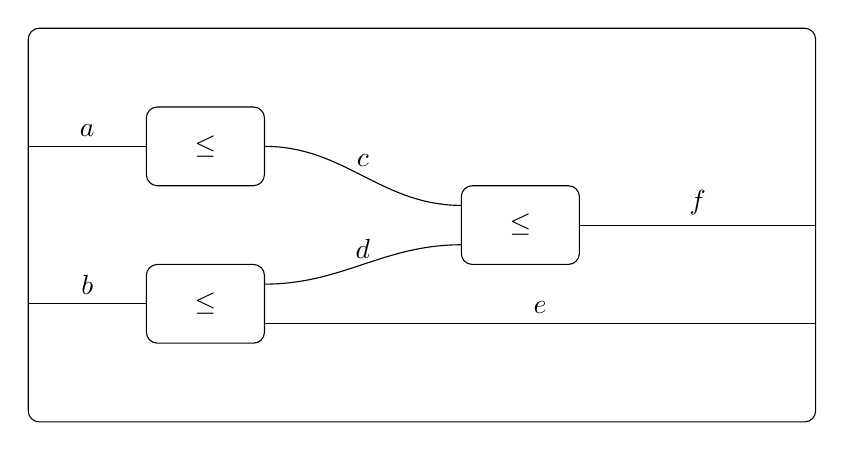
\begin{tikzpicture}[node distance={15mm}, main/.style = {draw, thick}]

\draw[rounded corners] (0, 0) rectangle (10, 5) {};
\draw[rounded corners] (1.5, 1) rectangle (3, 2) node[pos=0.5] {$\le$};
\draw[rounded corners] (1.5, 4) rectangle (3, 3) node[pos=0.5] {$\le$};
\draw[rounded corners] (5.5, 2) rectangle (7, 3) node[pos=0.5] {$\le$};

\draw (0, 3.5) -- (1.5, 3.5) node [midway, above] {$a$};
\draw (0, 1.5) -- (1.5, 1.5) node [midway, above] {$b$};
\draw (3, 1.25) -- (10, 1.25) node [midway, above] {$e$};

\draw (3, 3.5) edge[out=0,in=180] node[yshift=2mm] {$c$} (5.5, 2.75);
\draw (3, 1.75) edge[out=0,in=180] node[yshift=2mm] {$d$} (5.5, 2.25);

\draw (7, 2.5) -- (10, 2.5) node [midway, above] {$f$};

\end{tikzpicture}
